\paragraph{}

Simuler logiciellement le comportement d'un appareil tel que la NES nécessite de connaître précisément le fonctionnement de chacune des unités de traitement qui le constitue : leur architecture matérielle, les données qu'elles manipulent, les connexions entre ces différentes unités, etc.

\paragraph{}
Nous avons donc commencé ce projet par une phase collective de recherche sur le fonctionnement global de la NES afin d'acquérir une vision d'ensemble du système à émuler. Cela nous a permis d'acquérir un socle commun de connaissances sur le sujet.

\paragraph{}
C'est suite à ces recherches que nous avons pu établir une architecture logicielle appropriée puis une répartition des tâches au sein du groupe. Afin que chaque membre du projet se sente impliqué, cette répartition fut réalisée suivant les préférences de chacun. L'organisation des ressources humaines et temporelles furent retranscrites en un diagramme de Gantt. Sur ce diagramme ainsi que dans le cahier des charges, deux versions du projet ont été prévues : la première (v0) comportant les fonctions vitales à l'émulateur et une seconde (v1) ajoutant des fonctionnalités additionnelles.

\paragraph{}
Sur toute sa durée, ce projet fut ponctué de réunions d'équipe mais également de séances de travail de groupe, plus conséquentes, effectuées en amont de chaque grande étape du projet. Ces sessions de travail consistaient en une recherche d'informations approfondies sur les futures tâches pour que chacun ait une pleine compréhension des fonctionnalités a développer.

\paragraph{}
La gestion de ce projet s'est vu facilitée par l'utilisation du logiciel de versionning \emph{git}. Il nous a notamment permis de positionner chaque partie du projet sur des branches distinctes et ainsi de rendre sa gestion globale plus claire. Dans un premier temps, il a également été décidé d'utiliser un système de compilation par Makefile afin de mesurer son efficacité sur un tel projet. Par la suite, nous avons étendu ce système de compilation au Cmake dans l'optique de permettre à d'autre développeurs de configurer leur IDE avec le projet.

\begin{figure}[h]
  \centering
   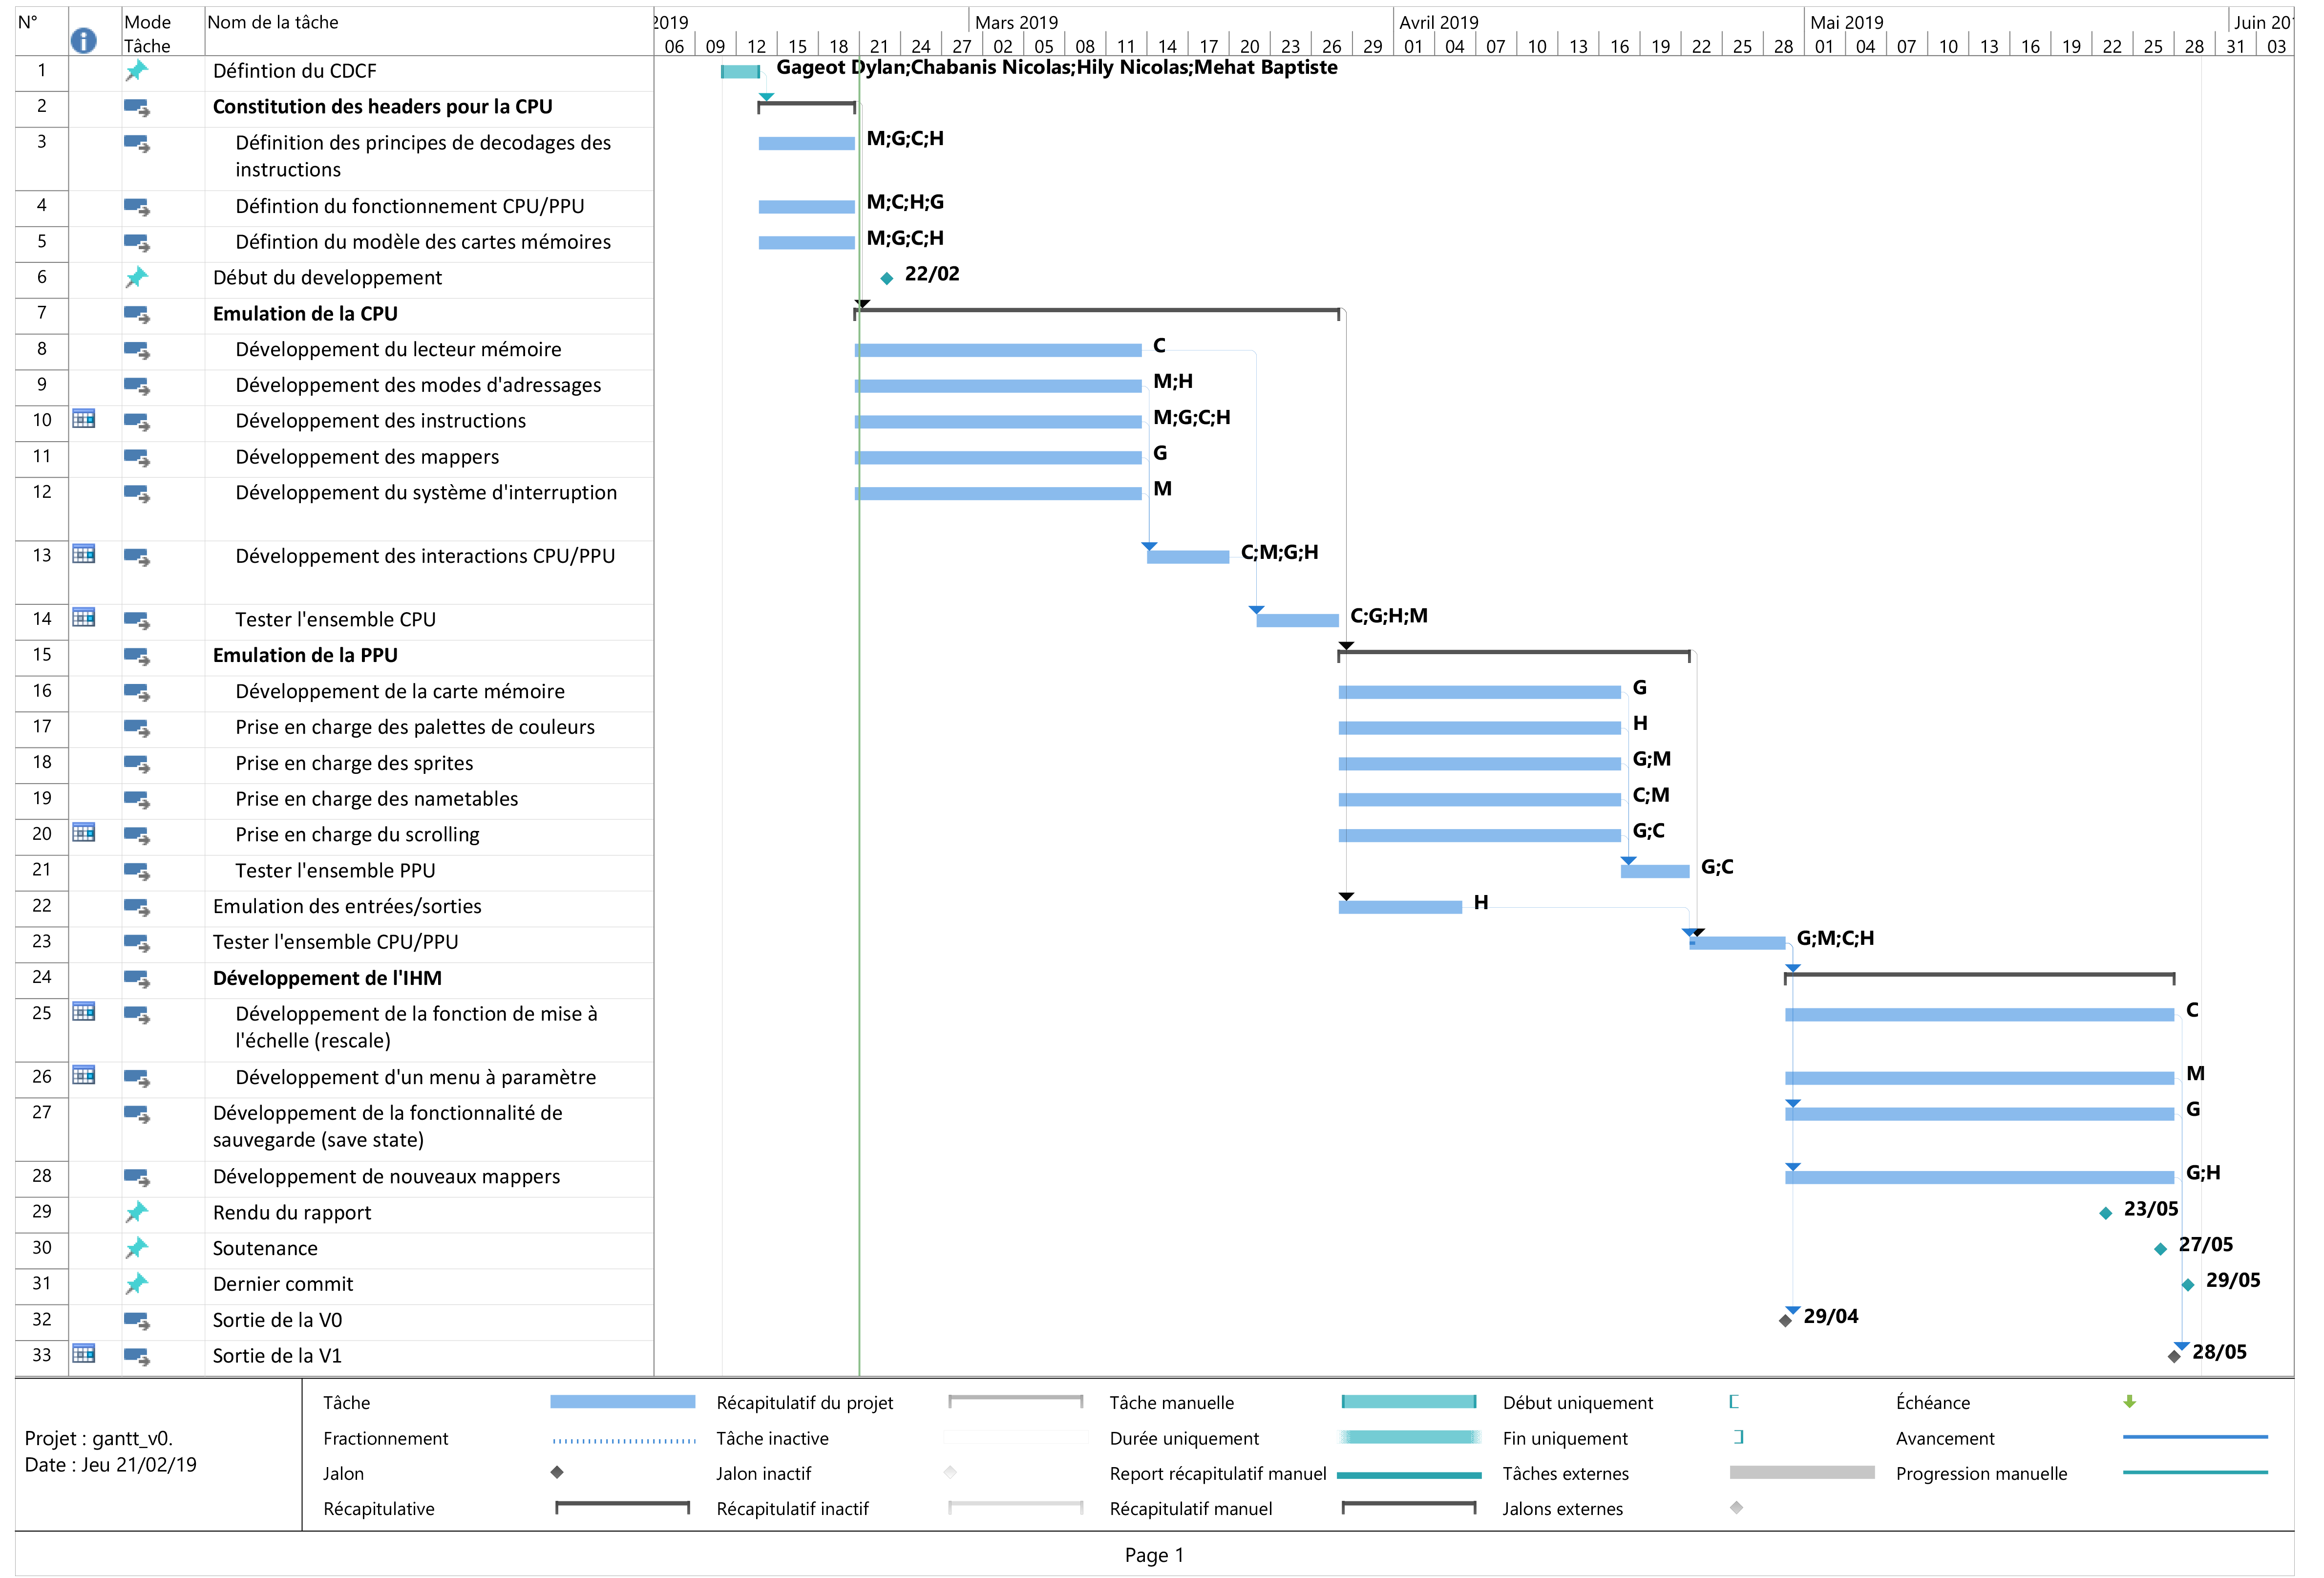
\includegraphics[scale=0.45]{GanttV1.png}
   \caption{\label{étiquette} Diagramme de Gantt de début de Projet}
\end{figure}
